\section{eo\-Vl\-Uniform\-Bin\-Op$<$ EOT $>$ Class Template Reference}
\label{classeo_vl_uniform_bin_op}\index{eoVlUniformBinOp@{eoVlUniformBinOp}}
Direct Uniform Exchange of genes for Variable Length, BINARY version.  


{\tt \#include $<$eo\-Variable\-Length\-Crossover.h$>$}

Inheritance diagram for eo\-Vl\-Uniform\-Bin\-Op$<$ EOT $>$::\begin{figure}[H]
\begin{center}
\leavevmode
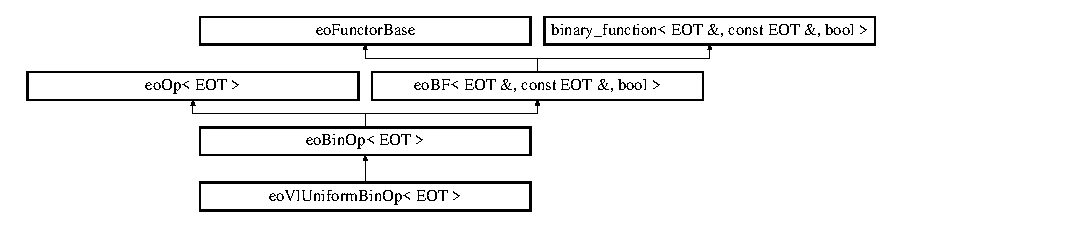
\includegraphics[height=2.60163cm]{classeo_vl_uniform_bin_op}
\end{center}
\end{figure}
\subsection*{Public Types}
\begin{CompactItemize}
\item 
typedef EOT::Atom\-Type {\bf Atom\-Type}\label{classeo_vl_uniform_bin_op_w0}

\end{CompactItemize}
\subsection*{Public Member Functions}
\begin{CompactItemize}
\item 
{\bf eo\-Vl\-Uniform\-Bin\-Op} (unsigned \_\-Min, unsigned \_\-Max, double \_\-rate=0.5)\label{classeo_vl_uniform_bin_op_a0}

\item 
bool {\bf operator()} ({\bf EOT} \&\_\-eo1, const {\bf EOT} \&\_\-eo2)\label{classeo_vl_uniform_bin_op_a1}

\begin{CompactList}\small\item\em The pure virtual function that needs to be implemented by the subclass. \item\end{CompactList}\end{CompactItemize}
\subsection*{Private Attributes}
\begin{CompactItemize}
\item 
unsigned {\bf Min}\label{classeo_vl_uniform_bin_op_r0}

\item 
unsigned {\bf Max}\label{classeo_vl_uniform_bin_op_r1}

\item 
double {\bf rate}\label{classeo_vl_uniform_bin_op_r2}

\end{CompactItemize}


\subsection{Detailed Description}
\subsubsection*{template$<$class EOT$>$ class eo\-Vl\-Uniform\-Bin\-Op$<$ EOT $>$}

Direct Uniform Exchange of genes for Variable Length, BINARY version. 

A very primitive version, that does no verification at all!!! NEEDS to be improved - but no time now :-((( Especially, if both guys have maximal size, it will take some time to generate even 1 offspring that is not oversized!!! Also, we should first check for identical atoms, and copy them to the offspring, and only after that exchange the other ones (Radcliffe's RRR). 



Definition at line 280 of file eo\-Variable\-Length\-Crossover.h.

The documentation for this class was generated from the following file:\begin{CompactItemize}
\item 
eo\-Variable\-Length\-Crossover.h\end{CompactItemize}
